% Sandia National Laboratories is a multimission laboratory managed and
% operated by National Technology & Engineering Solutions of Sandia, LLC, a
% wholly owned subsidiary of Honeywell International Inc., for the U.S.
% Department of Energy’s National Nuclear Security Administration under
% contract DE-NA0003525.

% Copyright 2002-2020 National Technology & Engineering Solutions of Sandia,
% LLC (NTESS).


\begin{Device}

\symbol
{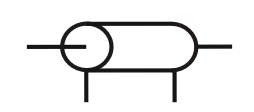
\includegraphics{translineSymbol}}

\device
\begin{alltt}
ytransline <name> <Input port> <Output port> testLine 
+ len=<value> lumps=<value>
\end{alltt}

\model
\begin{alltt}
.model testLine transline r=<value> l=<value> 
+ c=<value> [model parameters]
\end{alltt}

\examples
\begin{alltt}
ytransline line1 inn out  testLine len=12.0 lumps=1440
\end{alltt}

\comments
The lumped transmission line, device is a two port bi-directional device.   The specification
is patterned, loosely, from the netlist specification for the LTRA device.

\texttt{R}, \texttt{L}, and \texttt{C}  are the resistance,
inductance, and capacitance of the transmission line per unit
length, respectively. \texttt{LEN} is the total length of the transmission
line, and \texttt{LUMPS} is the number of lumped elements used to discretize the line. 
Supported configurations for this device are \texttt{RLC} and \texttt{LC}.

Unlike the LTRA device, which is based on an analytic solution, this device is 
based on assembling chains of linear R,L and C devices to approximate the 
solution to the Telegraph equations.  It is the functional equivalent of building a
transmission line in the netlist using subcircuits of linear elements.  The advantage
of using this approach is that it automates the mechanics of this process, and
thus is less prone to error.  It can be used with all analysis types, including
harmonic balance (HB).

The model is based on the assumption that the segments of the line are evenly spaced.
The number of segments is specified by the parameter \texttt{LUMPS} and the larger 
this number, the more accurate the calculation.
\end{Device}

\paragraph{Device Parameters}
% This table was generated by Xyce:
%   Xyce -doc Transline 1
%
\index{lumped transmission line!device instance parameters}
\begin{DeviceParamTableGenerated}{Lumped Transmission Line Device Instance Parameters}{Transline_1_Device_Instance_Params}
LEN & length of line & m & 0 \\ \hline
LUMPS &  & -- & 1 \\ \hline
\end{DeviceParamTableGenerated}


\paragraph{Model Parameters}
% This table was generated by Xyce:
%   Xyce -doc Transline 1
%
\index{lumped transmission line!device model parameters}
\begin{DeviceParamTableGenerated}{Lumped Transmission Line Device Model Parameters}{Transline_1_Device_Model_Params}
C & Capacitance per unit length & F/m & 0 \\ \hline
ELEV &  & -- & 2 \\ \hline
G & Conductance per unit length & $\mathsf{\Omega}^{-1}$ m$^{-1}$ & 0 \\ \hline
L & Inductance per unit length & Hm$^{-1}$ & 0 \\ \hline
R & Resistance per unit length & $\mathsf{\Omega}/$m & 0 \\ \hline
\end{DeviceParamTableGenerated}



%\paragraph{References}
%%See references \cite{Roychodhury:1994} and \cite{Spice3f5-user-guide} for more information
%about the model.
